%%%%%%%%%%%%%%%%%%%%%%%%%%%%%%%%%%%%%%%%%
% Thin Sectioned Essay
% LaTeX Template
% Version 1.0 (3/8/13)
%
% This template has been downloaded from:
% http://www.LaTeXTemplates.com
%
% Original Author:
% Nicolas Diaz (nsdiaz@uc.cl) with extensive modifications by:
% Vel (vel@latextemplates.com)
%
% License:
% CC BY-NC-SA 3.0 (http://creativecommons.org/licenses/by-nc-sa/3.0/)
%
%%%%%%%%%%%%%%%%%%%%%%%%%%%%%%%%%%%%%%%%%

%----------------------------------------------------------------------------------------
%	PACKAGES AND OTHER DOCUMENT CONFIGURATIONS
%----------------------------------------------------------------------------------------
\documentclass[12pt]{article} % Font size (can be 10pt, 11pt or 12pt) and paper size (remove a4paper for US letter paper)
\usepackage[protrusion=true,expansion=true]{microtype} % Better typography
\usepackage[left=1in,right=1in,top=.95in,bottom=.95in]{geometry}
\usepackage{graphicx} % Required for including pictures
\usepackage{wrapfig} % Allows in-line images
%\usepackage{mathpazo} % Use the Palatino font
\usepackage[T1]{fontenc} % Required for accented characters
%\linespread{1.05} % Change line spacing here, Palatino benefits from a slight increase by default
%\usepackage{array}
%\usepackage{booktabs}
%\usepackage{latexsym}
\usepackage{fancyhdr}
\usepackage{lastpage}
\usepackage[pdftex]{hyperref}
\usepackage{tipa}
\usepackage{url}
\usepackage{verbatim}
\hypersetup{
  colorlinks = true,
  urlcolor = black,
  citecolor=black,%
  filecolor=black,%
  linkcolor=black,%
  urlcolor=black     % can put red here to visualize the links
}
%\usepackage{biblatex}

\usepackage{outlines}
\usepackage{enumitem}
\usepackage{mathtools}
\usepackage{vector}
\usepackage{fixltx2e}

\usepackage{pdfpages}

\usepackage{xfrac}

\usepackage[labelfont=bf]{caption}

%\usepackage[latin1]{inputenc}
\usepackage{tikz}
\usetikzlibrary{shapes,arrows}


\newcounter{cenum}
\newcounter{cenumsaved}
\setcounter{cenumsaved}{0}
\newcommand{\labelcenum}{\arabic{cenum}.}
\newenvironment{cenumerate}%
{\begin{list}{\labelcenum}{\usecounter{cenum}}%
\setcounter{cenum}{\value{cenumsaved}}}%
{\setcounter{cenumsaved}{\value{cenum}}%
\end{list}}

\renewcommand{\outlineii}{cenumerate}

%\setenumerate[1]{label=\Roman*.}
%\setenumerate[2]{label=\Alph*.}
%\setenumerate[3]{label=\roman*.}
%\setenumerate[4]{label=\alph*.}

\makeatletter
%\renewcommand\@biblabel[1]{\textbf{#1.}} % Change the square brackets for each bibliography item from '[1]' to '1.'
\renewcommand{\@listI}{\itemsep=0pt} % Reduce the space between items in the itemize and enumerate environments and the bibliography

\renewcommand{\maketitle}{ % Customize the title - do not edit title and author name here, see the TITLE block below
\begin{center} % Right align
{\noindent\@title} % Increase the font size of the title

\vspace{10pt} % Some vertical space between the title and author name

{\noindent\@author}\\\@date

\vspace{10pt} % Some vertical space between the author block and abstract
\end{center}
}


\let\oldhat\hat
\renewcommand{\vec}[1]{\mathbf{#1}}
\renewcommand{\hat}[1]{\oldhat{\mathbf{#1}}}


\providecommand{\e}[1]{\ensuremath{\times 10^{#1}}}

%----------------------------------------------------------------------------------------
%	TITLE
%----------------------------------------------------------------------------------------
%\title{\LARGE{\textbf{Software Engineering Best Practices\\in Biomedical Informatics}\\[.5em]
%}}
%
%\author{\large{Nicholas J. Matiasz}\vspace{.4em}}
%
%\date{\large{2013-10-31}} % Date
%----------------------------------------------------------------------------------------

%----------------------------------------------------------------------------------------
%	HEADER/FOOTER
%----------------------------------------------------------------------------------------
\lhead{}
\chead{}
\rhead{}
\lfoot{BE 224A \textpipe\ MRI Lecture}
\cfoot{\thepage\ of\ \pageref{LastPage}}
\rfoot{Nicholas J. Matiasz}
\renewcommand{\headrulewidth}{0.4pt}
\renewcommand{\footrulewidth}{0.4pt}
\pagestyle{fancyplain}



%----------------------------------------------------------------------------------------
%	ESSAY BODY
%----------------------------------------------------------------------------------------
\begin{document}

\begin{titlepage}

\newcommand{\HRule}{\rule{\linewidth}{0.5mm}} % Defines a new command for the horizontal lines, change thickness here

\center % Center everything on the page
 
%----------------------------------------------------------------------------------------
%	HEADING SECTIONS
%----------------------------------------------------------------------------------------

\textsc{\Large University of California, Los Angeles}\\[1.5cm] % Name of your university/college
\textsc{\large Medical Imaging Informatics Group}\\[0.5cm] % Major heading such as course name
\textsc{\large BE 224A MRI Lecture}\\[0.5cm] % Minor heading such as course title

%----------------------------------------------------------------------------------------
%	TITLE SECTION
%----------------------------------------------------------------------------------------
\vspace{20pt}
\HRule \\[0.5cm]
\LARGE{\textbf{Lecture notes on the spin echo}}\\[.3cm]
\LARGE{\textbf{pulse sequence of MRI}}\\
\HRule \\[1.5cm]
 
%----------------------------------------------------------------------------------------
%	AUTHOR SECTION
%----------------------------------------------------------------------------------------

\begin{minipage}{0.4\textwidth}
\begin{flushleft} \large
\emph{Author:}\\
Nicholas J.\ Matiasz % Your name
\end{flushleft}
\end{minipage}
~
\begin{minipage}{0.4\textwidth}
\begin{flushright} \large
\emph{Instructor:} \\
Prof.\ Ricky Taira % Supervisor's Name
\end{flushright}
\end{minipage}\\[4cm]

% If you don't want a supervisor, uncomment the two lines below and remove the section above
%\Large \emph{Author:}\\
%John \textsc{Smith}\\[3cm] % Your name

%----------------------------------------------------------------------------------------
%	DATE SECTION
%----------------------------------------------------------------------------------------
\begin{minipage}{0.4\textwidth}
\begin{center} \large
\emph{Submitted:} \\
2014-02-18 % Supervisor's Name
\end{center}
\end{minipage}\\[4cm]
%{\large Submitted: 2013-10-30}\\[3cm] % Date, change the \today to a set date if you want to be precise

%----------------------------------------------------------------------------------------
%	LOGO SECTION
%----------------------------------------------------------------------------------------
%\includegraphics{Logo}\\[1cm] % Include a department/university logo - this will require the graphicx package
%----------------------------------------------------------------------------------------
\vfill % Fill the rest of the page with whitespace
\end{titlepage}


\fontsize{12}{19.416407865}%22.5, 28
\selectfont
%\thispagestyle{empty}
%\tableofcontents

\section{Introduction}
This text is a collection of lecture notes to explain the spin echo pulse sequence that is used for magnetic resonance imaging (MRI). 
The need for pulse sequences in MRI is first motivated, followed by a detailed explanation of the spin echo pulse sequence.

\section{Pulse sequences}
Although a complete description of MRI is beyond the scope of this text, it should be noted that a major source of image contrast in this modality is that tissues exhibit different magnetic properties based on a variety of factors, including molecular size and chemical composition. 
Pulse sequences, in the form of electromagnetic radiation in the radio frequency (RF) range, are used to perturb the imaged body. This strategy exposes the inherent differences that exist between the tissue's various media. 
The spin echo pulse sequence is an example of this strategic application of RF radiation.

\section{Spin echo}
Spin echoes in nuclear magnetic resonance were first explained in detail by Erwin Hahn in 1950 \cite{hahn1950a, hahn1950b}.
Carr and Purcell \cite{carr1954} introduced the technique of using a second pulse that is twice the duration of the first, as is explained below. Bushberg, et al. \cite{bushberg2002} synthesize many of these MRI-related concepts, and provide numerous illustrations of the spin echo pulse sequence (some of which are reproduced in this text). It should be acknowledged that much of the discussion below was derived from explanations in \cite{bushberg2002}.

\subsection{Pre-pulse state}
In a tissue, each proton's spin gives rise to a magnetic dipole moment, $\boldsymbol{\mu}$.
In the absence of an external magnetic field, these magnetic dipole moments are oriented randomly in space, such that the vector components of the spins statistically cancel each other, leaving no net magnetization vector. In the presence of a strong magnetic field (e.g., 1.5--3~T), $\vec{B_{0}}$, the spins assume known orientations. For quantum mechanical reasons, hydrogen protons in the presence of $\vec{B_{0}}$ can assume one of two possible states, which are called \textit{parallel} and \textit{anti-parallel}. Despite their names, these two states do not result in perfect alignment with or opposition to the direction of $\vec{B_{0}}$---again for quantum mechanical reasons regarding the quantization of space.

The parallel state is a lower-energy state than the anti-parallel state. For this reason, the vast majority of hydrogen protons assume the parallel state in the presence of $\vec{B_{0}}$. The proportion of protons that assume the anti-parallel state depends on the difference in energy between these two states, $\Delta E$, as well as on the temperature, $T$, of the tissue. The ratio of the number of parallel protons, $N_{2}$, to the number of anti-parallel protons, $N_{1}$, is given by Equation \ref{eq:spin_up_spin_down}, where $k$ is the Boltzmann constant.

\begin{equation}
\frac{N_{2}}{N_{1}} = e^{-\frac{\Delta E}{kT}}
\label{eq:spin_up_spin_down}
\end{equation}

When $\vec{B_{0}}$ is applied and the protons assume the parallel and anti-parallel states, the magnetic dipole moments of the spins are no longer oriented randomly in space. If the $z$-axis is set to be the direction of $\vec{B_{0}}$, the $z$-vector components of the spins' magnetic dipole moments now sum to give a non-zero net magnetization vector, $\vec{M_{0}}$, as shown in Equation \ref{eq:net_magnetization}, and as depicted in Figure \ref{fig:spins_in_b0}-B.

\begin{equation}
\vec{M_{0}} = \sum\limits_{i=1}^N\boldsymbol{\mu}_{i}
\label{eq:net_magnetization}
\end{equation}

\begin{figure}[h]
\centering
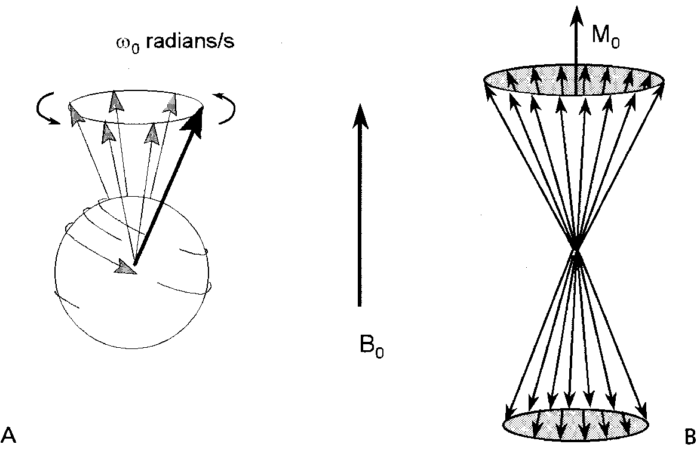
\includegraphics[scale=0.75]{./images/spins_in_b0.png}
\caption{\textbf{A}: An illustration of the Larmor frequency. \textbf{B}: The net magnetization vector that occurs in the presence of $\vec{B_{0}}$ \cite{bushberg2002}.}
\label{fig:spins_in_b0}
\end{figure}

In this configuration, $\vec{M_{0}}$ is collinear with the $z$-axis; in other words, it has no component in the $xy$-plane, even though each spin is tilted slightly away from the $z$-axis.
Despite having a fixed angle with respect to the $z$-axis, the parallel and anti-parallel spins are still precessing around the $z$-axis, such that they trace two circles in the $xy$-plane, as shown in Figure \ref{fig:spins_in_b0}-B.
This movement is analogous to that of a spinning top, which---due to the force of gravity---precesses on a table when it is tilted (i.e., not perfectly upright). 
The angular precession frequency, $\omega_{0}$, is given by the element's gyromagnetic ratio, $\gamma$, in units of radians per second per tesla, and by the strength of the applied magnetic field, $B_{0}$, as shown in Equation \ref{eq:larmor}. 

\begin{equation}
\omega_{0} = \gamma B_{0}
\label{eq:larmor}
\end{equation}

The phases of the precessing spins are random, so the magnetic dipole moments' components in the $xy$-plane statistically cancel, yielding a $\vec{M_{0}}$ that is collinear with the $z$-axis, and whose magnitude depends on the ratio presented in Equation \ref{eq:spin_up_spin_down}. At this point, the system is ready for a spin echo pulse sequence to manifest a nuclear magnetic resonance signal.

\subsection{90-degree pulse}
As mentioned above, the spin echo pulse sequence is delivered in the form of RF energy---specifically, two RF pulses of finite durations, the first of which is called the 90-degree pulse. The energy of these RF signals must be matched to the angular precession frequency, $\omega_{0}$, which is also related to the difference in energy between the parallel and anti-parallel states. Ensuring that the RF energy is matched to $\omega_{0}$ produces a resonance phenomena in which a portion of the parallel protons switch to the anti-parallel state. Additionally, the RF signal causes the phases of the spins to align; the $xy$-components of the magnetic dipole moments no longer statistically cancel, and $\vec{M_{0}}$ gains a non-zero component in the $xy$-plane.

The net effect of these events is that the net magnetization vector gets tipped toward the $xy$-plane until its $z$-component becomes zero, and its $xy$-component reaches a maximum, as depicted in Figure \ref{fig:spin_echo_overview}. This effect is what gives the 90-degree pulse its name. In the classical sense, the applied RF pulse has a sinusoidally-varying magnetic component. From the perspective of a rotating frame (see Figure \ref{fig:spin_echo_overview}), a component vector of this magnetic field is not moving with respect to the protons in the tissue, because the applied RF pulse has a frequency that is equal to the Larmor frequency. This magnetic signal, detected by a coil near the tissue, exhibits the behavior depicted in Figures \ref{fig:fid} and \ref{fig:spin_echo_overview}, known as the free induction decay (FID) \cite{bushberg2002}. The FID signal oscillates at the Larmor frequency, and decays at a rate that is dependent on the characteristics of the tissue. The decay occurs due to the gradual loss of phase coherence among the spins, which itself occurs due to magnetic inhomogeneities in the tissue.

\begin{figure}[h]
\centering
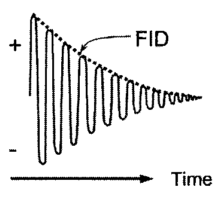
\includegraphics[scale=1.0]{./images/fid.png}
\caption{Free induction decay (FID) signal \cite{bushberg2002}}
\label{fig:fid}
\end{figure}

\subsection{180-degree pulse}
If an eventual spin echo (explained below) will occur at time TE, the 180-degree RF pulse is administered to the system at time TE/2. Like its 90-degree counterpart, the 180-degree pulse also rotates the net magnetization vector---but this time by 180 degrees instead of only 90 degrees. Bushberg, et al. \cite[p. 391--2]{bushberg2002} provide great clarity on this point via an instructive analogy, which refers to the diagrams of Figures \ref{fig:spin_echo_overview} and \ref{fig:spin_echo_signal}:
\begin{quote}
The B\textsubscript{0} inhomogeneity-canceling effect that the spin echo pulse sequence produces has been likened to a foot race on a track. The racers start running at the 90-degree pulse, but quickly their tight grouping at the starting line spreads out (dephases) as they run at different speeds. After a short period, the runners are spread out along the track, with the fastest runners in front and the slower ones in the rear. At this time (TE/2), a 180-degree pulse is applied and the runners all instantly reverse their direction, but they keep running at the same speed as before. Immediately after the 180-degree rephasing RF pulse, the fastest runners are the farthest behind and the slowest runners are in front of the pack. Under these conditions, the fast runners at the end of the pack will catch the slow runners at the front of the pack as they all run past the starting line together (i.e., at time TE). Even in a field of runners in which each runs at a markedly different speed from the others, they all will recross the starting line at exactly TE. The MR signal is at a maximum (i.e., the peak of the FID) envelope as the runners are all in phase when they cross the starting line.
\end{quote}

\begin{figure}[h]
\centering
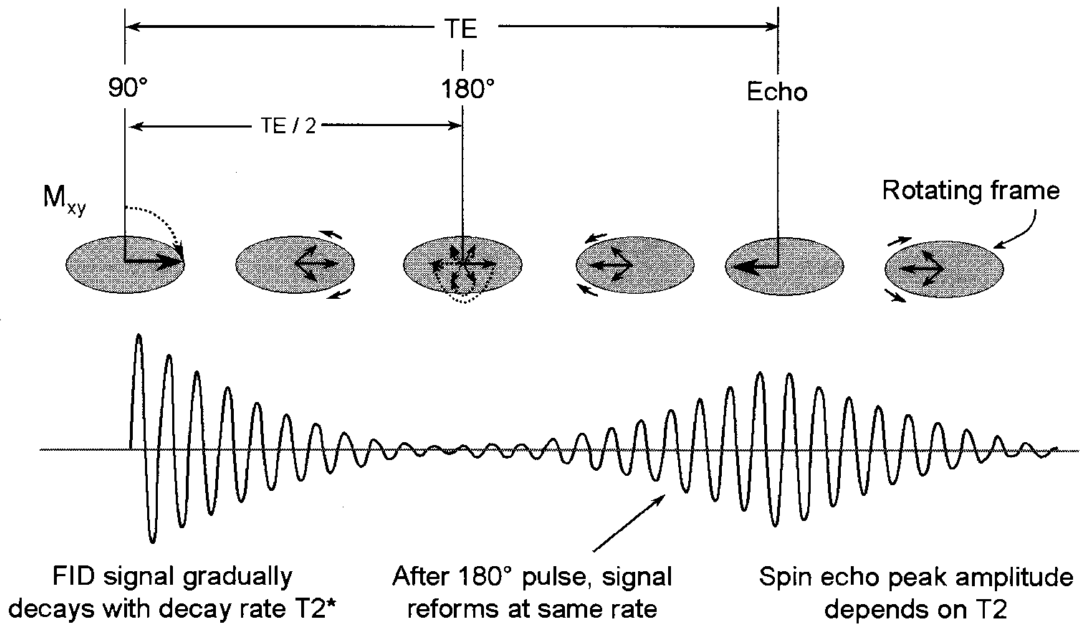
\includegraphics[scale=0.6]{./images/spin_echo_overview.png}
\caption{Overview of spin echo pulse sequence \cite{bushberg2002}}
\label{fig:spin_echo_overview}
\end{figure}

\begin{figure}[h]
\centering
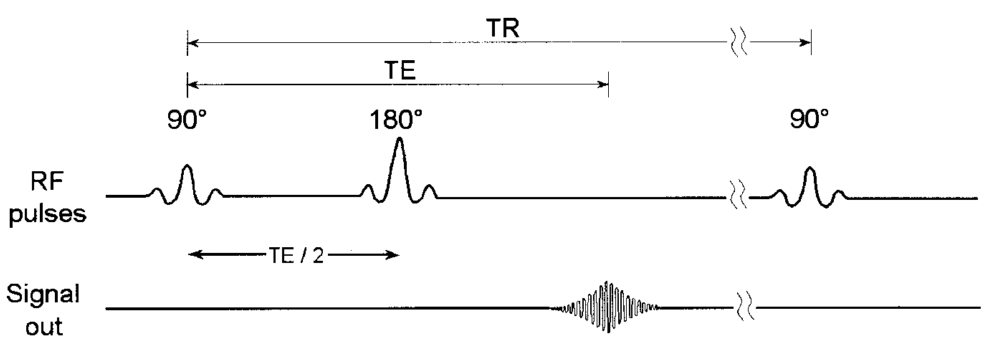
\includegraphics[scale=0.6]{./images/spin_echo_signal.png}
\caption{Signal generated by spin echo sequence \cite{bushberg2002}}
\label{fig:spin_echo_signal}
\end{figure}

\subsection{Post-pulse echo}
As the above analogy explains, the 180-degree RF pulse causes a phase reversal at time TE/2. After another interval of duration TE/2 (i.e., at time $2\frac{\text{TE}}{2} = \text{TE})$, the phase differences that arose gradually have had sufficient time to once again cohere, and this repeated establishment of phase coherence produces an echo of the original FID signal. The generation of this signal can be further understood by referring to Figure \ref{fig:spin_echo_overview} and noticing the correlation between the amplitude of the FID signal and the extent to which the spin vectors exhibit phase coherence. Figure \ref{fig:spin_echo_signal} depicts the signal that results from the spin echo pulse sequence, and also shows TR, the time interval between applications of 90-degree pulses. As this diagram suggests, the spin echo pulse sequence is repeated multiple times to further discriminate between different regions of tissue.

\section{Summary}
The spin echo pulse sequence demonstrates how specific applications of RF energy perturb the magnetic state of the tissue. These perturbations produce responses that can be measured, and the characteristics of the measured signals depend on the magnetic properties of the various tissue in the imaged body. These varying properties give rise to the image contrast in MRI. Pulse sequences are used in conjunction with spatial localization techniques to build a complete picture of the imaged body.

%----------------------------------------------------------------------------------------
%	BIBLIOGRAPHY
%----------------------------------------------------------------------------------------
%\newpage
\bibliographystyle{plain}
\bibliography{224a_pulse_sequence_lecture}
%----------------------------------------------------------------------------------------

\end{document}